\documentclass[]{article}
\usepackage{lmodern}
\usepackage{truncate}
\usepackage{caption}
\usepackage{tocloft}
\usepackage{amssymb,amsmath}
\usepackage{ifxetex,ifluatex}
\usepackage{fixltx2e} % provides \textsubscript
\usepackage{longtable}
\usepackage{graphicx}
\usepackage[table]{xcolor}


\setlength{\parindent}{0pt}
\setlength{\parskip}{6pt plus 2pt minus 1pt}
\setlength{\emergencystretch}{3em}  % prevent overfull lines
\setcounter{secnumdepth}{0}

\usepackage[breaklinks=true]{hyperref}
\hypersetup{colorlinks,%
citecolor=blue,%
filecolor=blue,%
linkcolor=blue,%
urlcolor=blue}
\usepackage{url}
\usepackage{caption}
\usepackage{cleveref}
\usepackage{booktabs}
\usepackage{fancyvrb}
\usepackage[english]{babel}
\usepackage{geometry}
\geometry{verbose,letterpaper,tmargin=1in,bmargin=1in,lmargin=1in,rmargin=1in}

\usepackage{titlesec, blindtext, color}
\definecolor{gray75}{gray}{0.75}
\newcommand{\hsp}{\hspace{20pt}}

% Headers and page numbering
\usepackage{fancyhdr}
\pagestyle{fancy}
\lhead{  \nouppercase  \leftmark}
\rhead{\thepage}
\cfoot{}

% titles
\usepackage{titling}
\pretitle{\Large}
\posttitle{ \\}
\preauthor{\large}
\postauthor{}
\predate{\large}
\postdate{}

% figure float
\usepackage{float}
\floatplacement{figure}{h}
\usepackage{morefloats}

% section titles
\usepackage{sectsty}
\setcounter{secnumdepth}{2}
\usepackage[normalem]{ulem}
\sectionfont{\rmfamily\large}
\subsectionfont{\rmfamily\upshape\normalsize}
\subsubsectionfont{\rmfamily\normalsize}

% natbib
\usepackage[square, numbers]{natbib}
\bibliographystyle{unsrtnat}

% line spacing
\usepackage{setspace}
\linespread{1.2}
\raggedbottom


% define title
\title{Committee Report 2020}
\author{Michael David Catchen}
\date{}

\begin{document}

\maketitle

\vspace{3em}
\subsubsection*{Abstract}

As Anthropogenic activity rapidly reshapes our planet, forecasting the future of Earth's ecosystems and the services they provide humanity poses an immense but necessary challenge. 

The infrastructure for the collection and assimilation of the data required to model ecosystems at global scales is still in its infancy. Furthermore, robust prediction has long evaded ecological processes due to their inherently complex, stochastic, and emergent nature.


Many disciplines that deal with similarly complex phenomena have benefited from using simulation models as tools for both inference and prediction, but in this realm, ecology has been a slow adopter.

There is much to be gained in biodiversity science from the further adoption of these methods as regular.

Here, we outline the potential for generative simulation models in metacommunity ecology, both for answering fundamental questions about the structure of ecological communities in space and time, but also for application in the management of real systems facing climatic and land-use change.


We discuss how simulation models can be used to make predictions with real data, and then
describe a process-based model of metacommunity dynamics (based around \citep{vellend_conceptual_2010, poisot_beyond_2015, thompson_process-based_2020}), and detail how we'll implement this model as software that is modular and can be used to answer a variety of questions about metacommunity dynamics, both in the ``virtual laboratory" case \citep{railsback_agent-based_2011}, as well in empirical systems.
At the moment, there do not exist software tools that exist explicitly for the purpose of forecasting community structure under a given model of future climate and land use, and building and applying this type of software is the primary goal of the dissertation.
We then conclude by outlining the structure of the proposed chapters.  
    
    
\clearpage

{
\hypersetup{linkcolor=black}
\setcounter{tocdepth}{3}
\normalfont
\tableofcontents
}
\clearpage
\section{Introduction}

Humans have long sought to forecast natural phenomena. For ages, people have attempted to predict the weather, the movement of celestial bodies,  eclipses, natural disasters, and plagues---all largely unsuccessful aside from the occasional false positive. The principles used to develop predictions about the world have varied widely, yet of the numerous methods attempted thus far, quantitative models have proven ``unreasonably effective" in predicting the behavior of (some) systems \cite{unreas}. 
It is clear that some types of systems are more "forecastable" than others. For example, Edmund Halley's by-hand computations enabled him to predict the return of his eponymous comet 53 years in advance, and modern astrodynamics models can forecast eclipses down to (spatial resolution and temporal resolution here). However, predicting the weather or ecology at those timescales is unreasonable.     


We know that not all systems can be accurately forecasted if there is even minuscule measurement error \cite{chaos}.
Why is this? 


Historically, the process of developing a quantitative model has been one of \textit{reductionism}: a system is divided into parts, and those parts subdivided into parts further until no more subdivision is possible, at which point we study the atomic parts the our system in order to build our understanding from the ``bottom-up". There are good reasons for this---the limitations of analytical mathematics make high-dimensional representations of a system intractable, and therefore reducing a model to as few measurable values as possible was necessary to interface with the quantitative tools of the time. 

Of course, in reality every natural system is complex. 








Since Halley's time, the problem solving strategy of starting with the simplest case and gradually building toward a higher fidelity representation of the system has become a ubiquitous tool across the sciences \cite{polya_how_2009}.

There are good reasons for this---the limitations of analytical mathematics make high-dimensional representations of a system intractable, and therefore reducing a model to as few measurable values as possible was necessary to interface with the quantitative tools of the time. Of course, in reality every natural system is complex.
The motion of matter is subject to the ever-changing pairwise gravitational forces of all other matter in existence, and yet Halley was successful in predicting the dynamics of his comet by considering only a small subset of those interactions.
Not only that, but Newtonian mechanics adds the additional abstraction of representing the state of each object with only two values, position and momentum. Surely if one were to study the distribution of matter within the Sun, describing it as a single point at its center would seem overzealous. Yet, this abstraction did not invalidate Halley's model because the effects of internal heterogeneity are practically immeasurable on the scale of the entire system \cite{levins_dialectical_1987}.

Simulation models bridge the gap between conventional statistical approaches and machine learning models because they provide information about process. 


\section{My Background(?)}

I don't know very much about biology. I spent the first
two years of undergrad in the engineering school, and by the time I moved into the ecology and evolutionary biology department in my third year, I was already focused on a specific research project as part of a BA/MA. How did I end up studying ecology? In reverse, it is clear I was always interested in modeling systems.

Master's project
- what was it
- what did i read as part of it

Gaps in literature I've read

\section{Proposed Dissertation Structure}

Here, we propose the following four chapters:
First, a review of the relevant literature surrounding the core topics of the dissertation: spatial ecology, ecological networks, and forecasting. Second, a framework for forecasting the structure of ecological networks. Third, an investigation of the forecasting horizon for complex ecological networks. And finally, a framework and software toolkit for designing the spatial structure of landscapes to mitigate biodiversity loss, using the framework from the previous chapters.

\subsection{Chapter One --- Introduction and Review}

This chapter aims to introduce the subject of the dissertation and summarize the relevant work from the literature that will be built upon in the following chapters. The topics covered roughly fall into the categories
\begin{enumerate}
    \item Models and Inference in Ecology 
        \begin{itemize}
            \item What is a model? \cite{jaynes, crutchfeld}
            \item What are the different purposes models serve? 
            \item What types of models do ecologists commonly use? 
            \item What are their limitations? 
        \end{itemize}
    
    \item Spatial Ecology
        \begin{itemize}
            \item Theory of Island Biogeography 
            \item Metapopulation Theory
            \item Landscape Genetics and Resistance Surfaces
            \item SDMs
        \end{itemize} 
    
    \item Ecological Networks
        \begin{itemize}
            \item Complexity and Stability 
            \item Metacommunities (leibold 2003, velland 2010)
            \item Community Dynamics  
            \item Network Theory
        \end{itemize}
    \item Forecasting
        \begin{itemize}
            \item The Forecasting Problem
            \item Ecological Forecasting and Adaptive Management
        \end{itemize}
\end{enumerate}


\clearpage
\subsection{Chapter Two --- A Framework for Forecasting Ecological Networks}

This chapter outlines a framework for forecasting the structure of ecological networks. First, a survey of the sources of data. Models must interface with observables. 

The flow from data, through many possible choices of models, to a forecasted outcomes. 
Motivate why we need this, why incorporating interactions into forecasting models is necessary 

\subsection{Chapter Three --- The Forecasting Horizon of Complex Ecological Networks}

Forecasting inevitably operates on a specific timescale. On some timescales, forecasting ecological systems is trivial \cite{crutchfeld}.


The spatial and temporal resolution limits of forecasting. 
How much data? How much measurement error?

There is no measurement that can be made without uncertainty. This has profound implications for the utility of forecasts as the error in measurement of the state of a system inevitably will result in a forecast that diverges from reality at some point in the future. This is in the ideal case where the exact dynamics driving the observed reality is known.

For example, consider a double-pendulum---a classic example of chaotic dynamics. 



\begin{figure}[h]
    \centering
    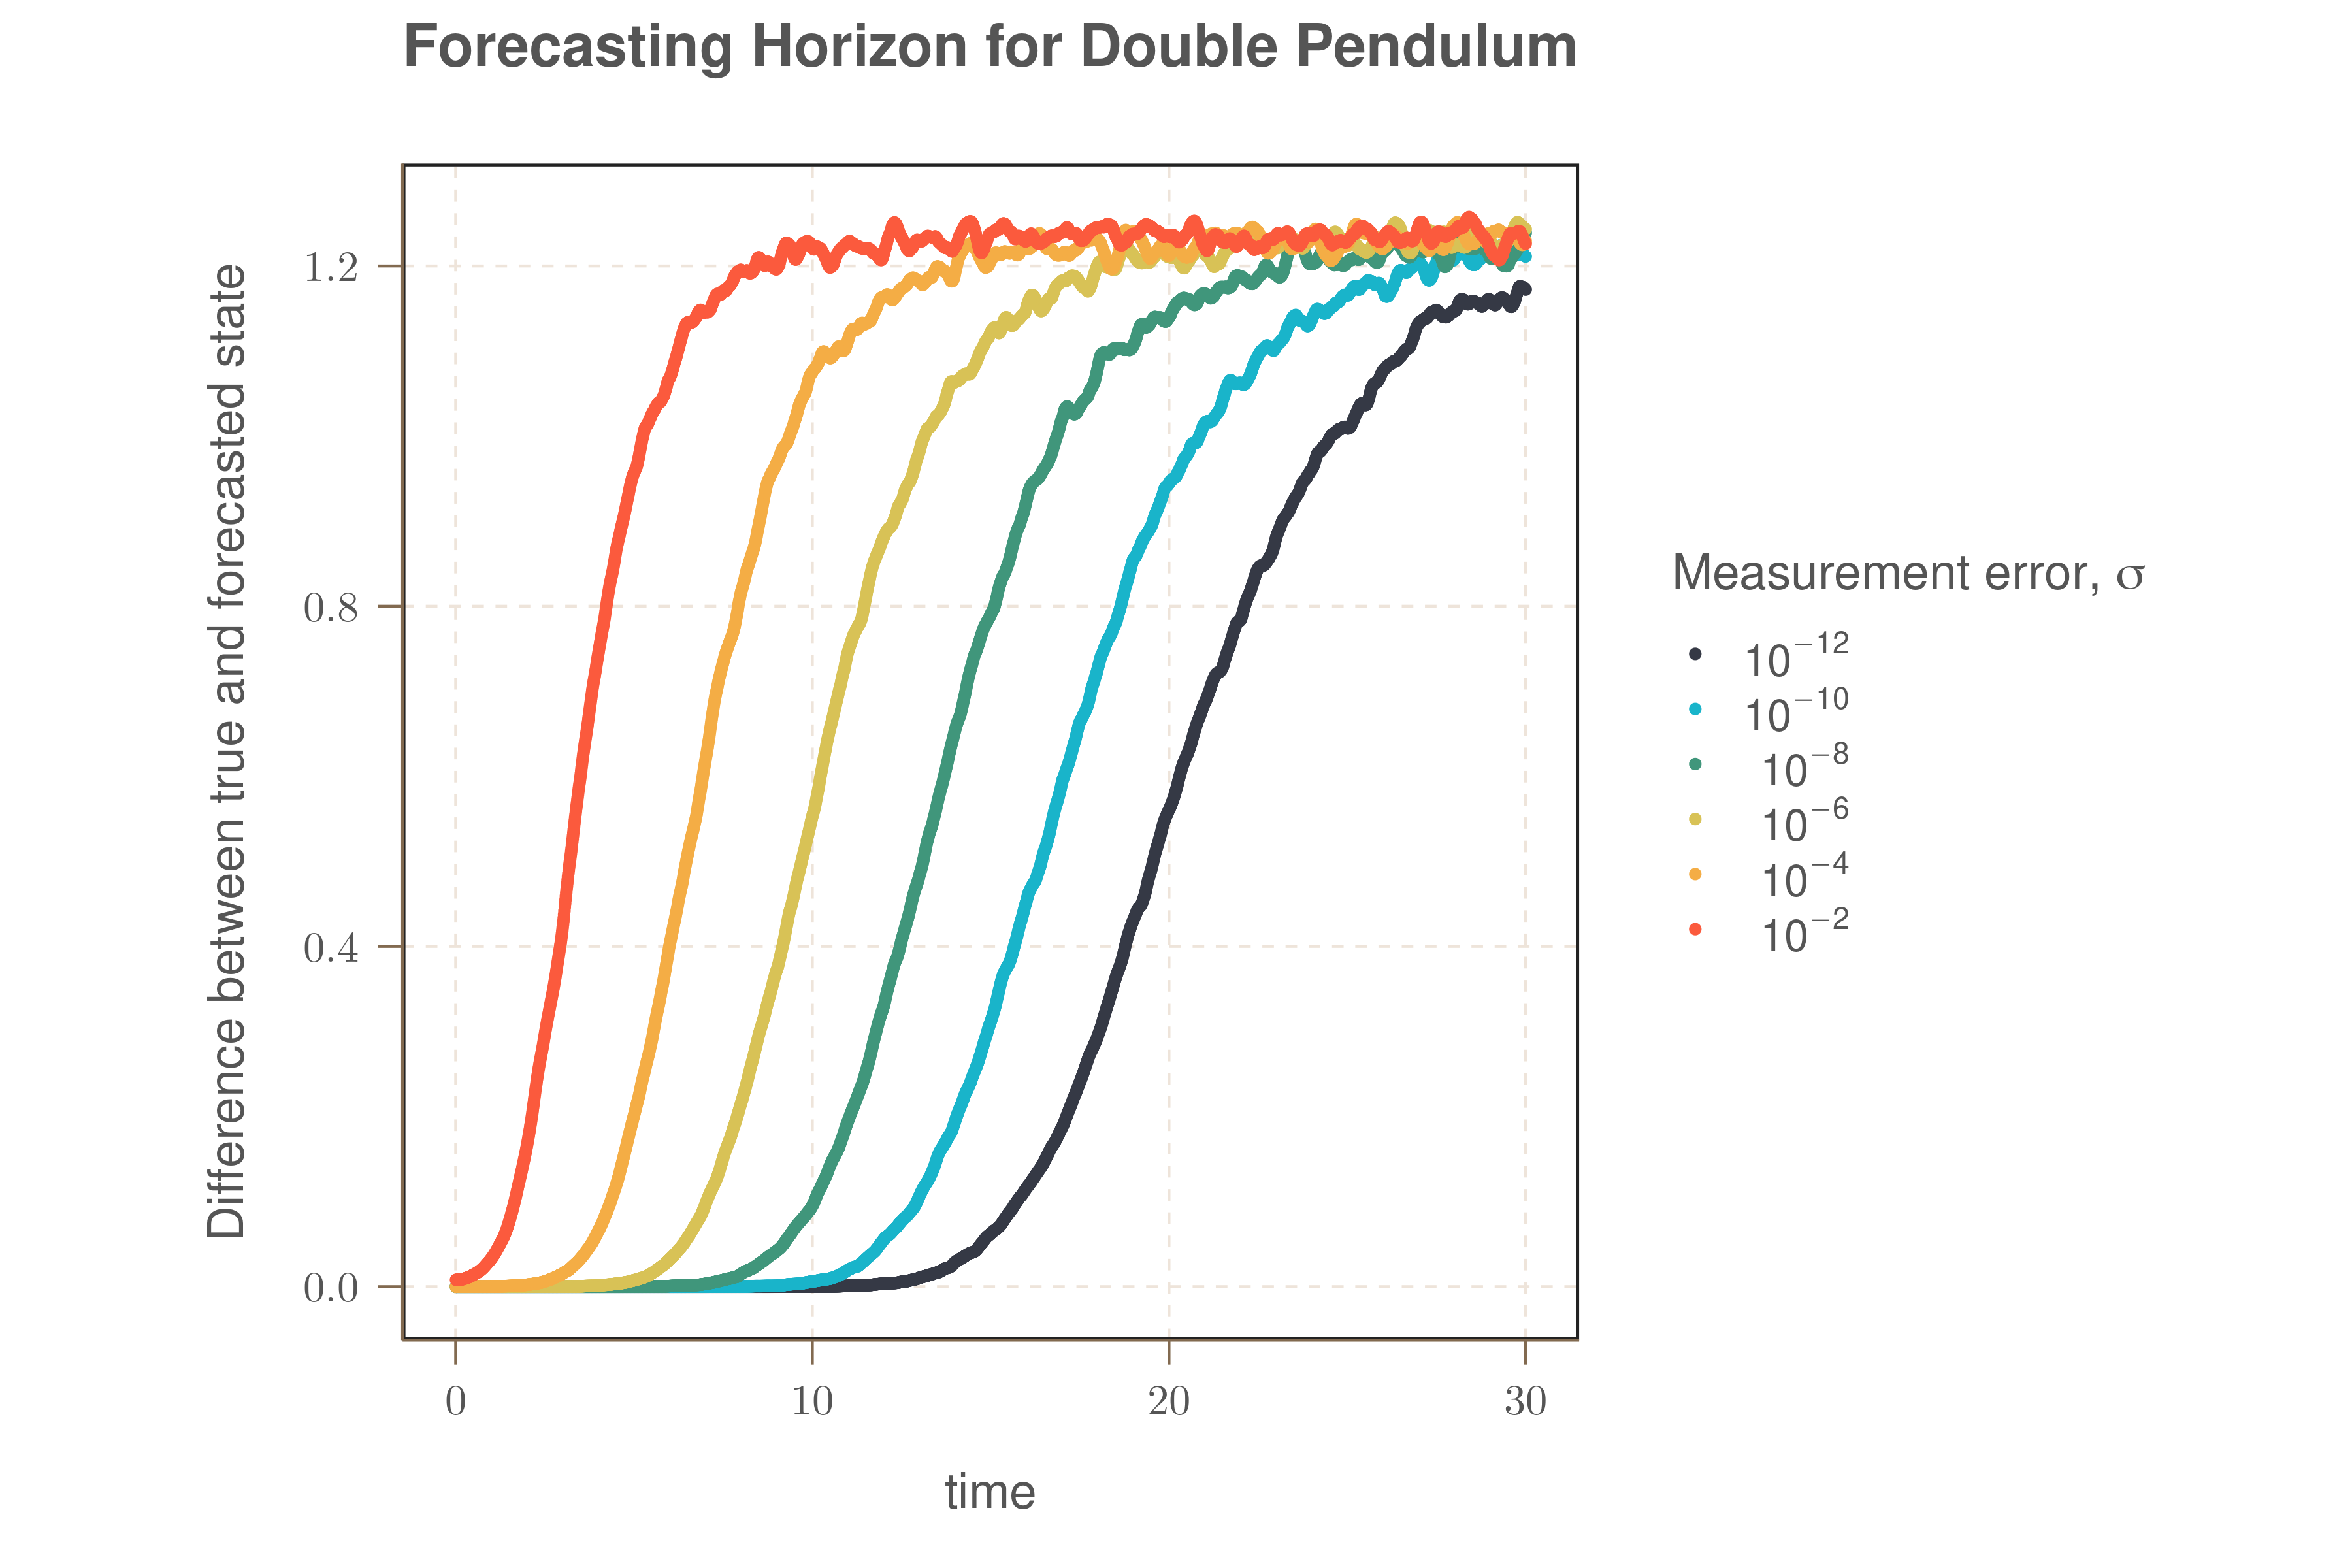
\includegraphics[width=17cm]{figs/forecasting_horizon.png}
    \caption{The error in a forecast of a double pendulum's position at various levels of inherent measurement error, $\sigma$. For 2000 replicates, a double pendulum was simulated with true initial condition $\{ \theta_1, \theta_2 \}$ and measured initial condition $\{\theta_A, \theta_B \}$}.
    \label{fig:forecasting_horizon}
\end{figure}


\subsection{Chapter Four --- Optimization models for designing landscapes to mitigate biodiversity loss under constraints }

Why are we interested in forecasting? One perspective is that the most powerful method of validating a scientific model is if it makes accurate predictions about the future. Good out-of-sample prediction is often the goal of building a machine learning model.

However, forecasting also has immediate practical value as a tool for planning to mitigate biodiversity loss and its impact on humanity.

In this context, the purpose of a forecast shifts dramatically. 

Forecast in order to decide on how best to intervene. 
Decision theory. 



\clearpage
\section{Proposed Timeline}
\begin{table}[H]
\begin{tabular}{lll}
Month          & Work  & Deliverables \\ \hline
November 2020  & Draft Forecasting Networks Paper, Finish revisions of Masters paper &                                   \\
December 2020  &                                                                     & Submitted Master's Paper          \\
January 2021   &                                                                     &                                   \\
February 2021  &                                                                     & Submit                            \\
March 2021     &                                                                     &                                   \\
April 2021     &                                                                     &                                   \\
June 2021      &                                                                     &                                   \\
July 2021      &                                                                     &                                   \\
August 2021    &                                                                     &                                   \\
September 2021 &                                                                     &                                   \\
October 2021   &                                                                     &                                  
\end{tabular}
\end{table}
\section{Figures}

\section{Tables}


\end{document}